\subsubsection{Giao diện người dùng - Danh sách hồ sơ đã ứng tuyển}

Người dùng có thể xem lại các hồ sơ ứng tuyển của họ cho từng công việc:

\begin{figure}[H]
    \centering
    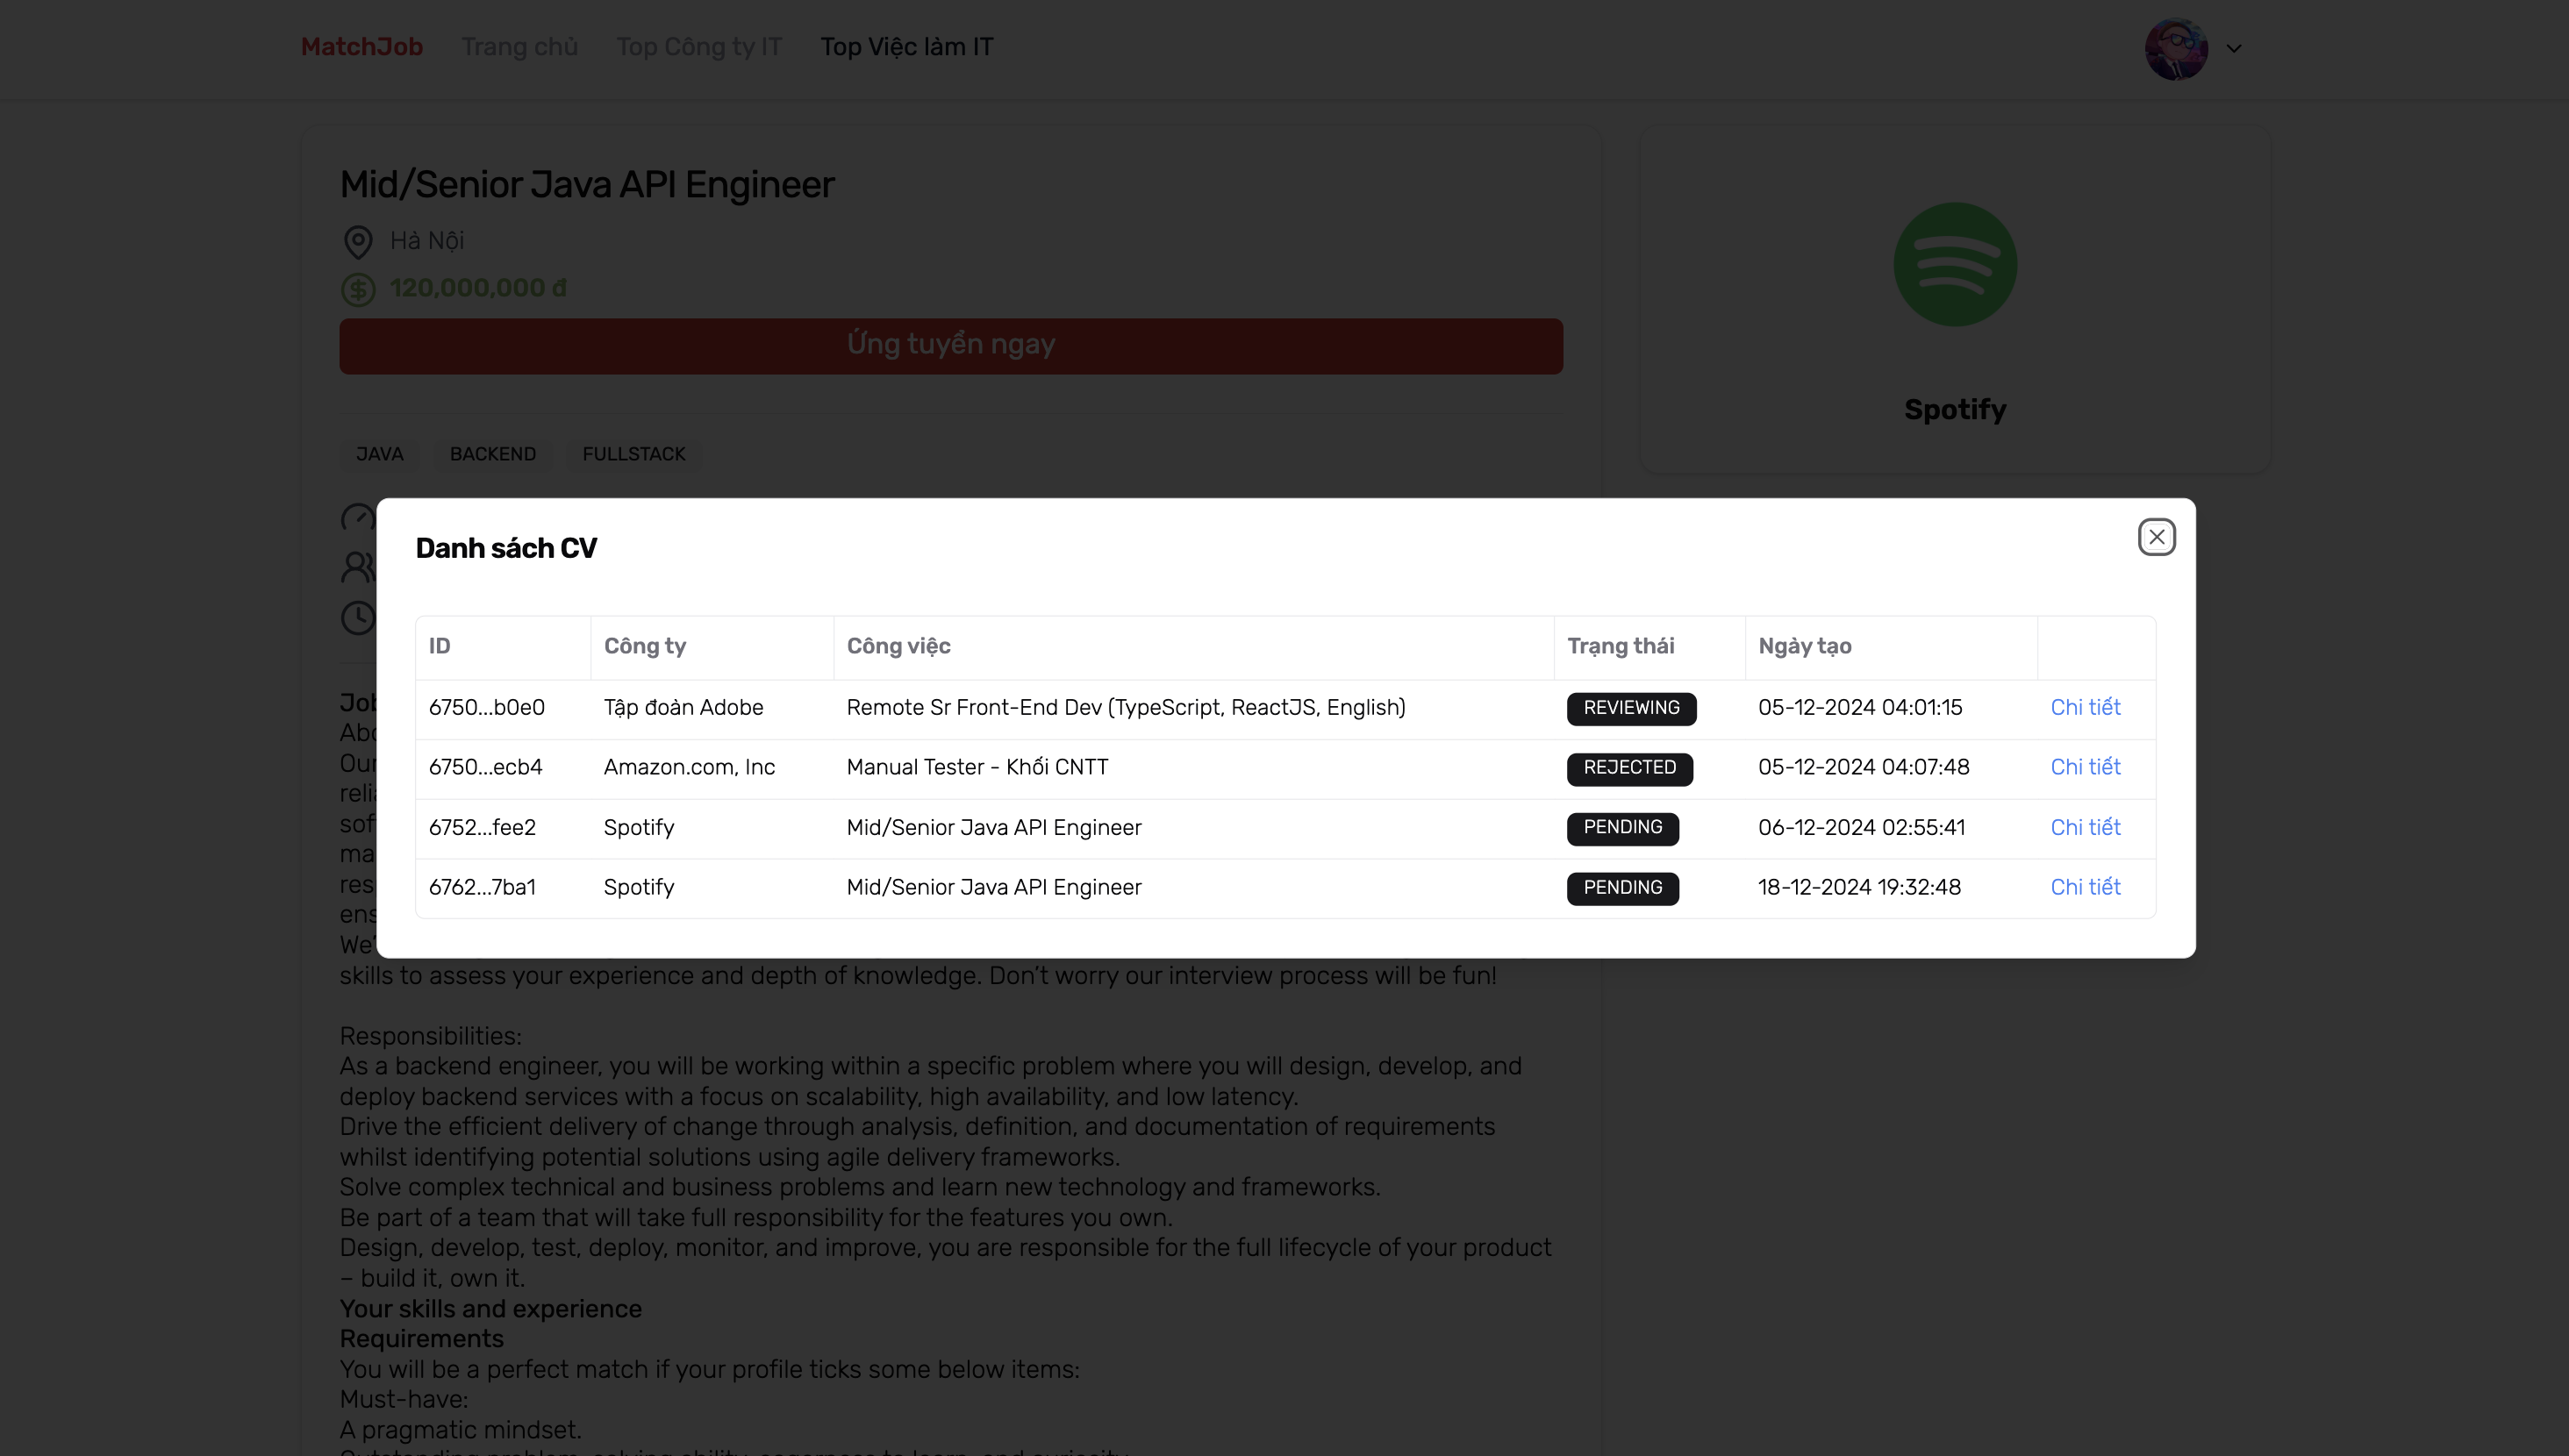
\includegraphics[width=\linewidth]{DBMS-Application/Images/modal-list-cv.png}
    \caption{Các hồ sơ đã được nộp của một người dùng}
\end{figure}

Truy vấn sử dụng:
\begin{itemize}
    \item \textbf{Query with join}: Sử dụng \texttt{\$lookup} để liên kết dữ liệu giữa hai collection \textbf{users} và \textbf{resumes}

    \item \textbf{Query with single condition}: Sử dụng \texttt{\$match} để lọc hồ sơ của của người dùng có \texttt{\_id}
\end{itemize}

\begin{lstlisting}
const result = await this.db
  .collection('users')
  .aggregate([
    {
      $lookup: {
        from: 'resumes',
        localField: '_id',
        foreignField: 'userId',
        as: 'userResumes',
      },
    },
    {
      $match: {
        _id: new ObjectId(user._id),
      },
    },
    {
      $project: {
        userResumes: 1,
      },
    },
  ])
  .toArray();

const resumes = result.length > 0 ? result[0].userResumes : [];
return resumes;
\end{lstlisting}

Giải thích truy vấn:
\begin{itemize}
    \item \texttt{\$lookup}: Thực hiện join giữa collection \textbf{users} và collection \textbf{resumes} để lấy tất cả các hồ sơ ứng tuyển của người dùng (\texttt{userId}) tương ứng với \texttt{\_id} của user.
    \item \texttt{\$match}: Lọc để chỉ lấy hồ sơ ứng tuyển của người dùng có \texttt{\_id} trùng với ID của user được truyền vào (\texttt{user.\_id}).
    \item \texttt{\$project}: Chỉ giữ lại trường \texttt{userResumes} trong kết quả trả về, ẩn các trường khác.
\end{itemize}

Truy vấn trả về mảng các hồ sơ ứng tuyển (\texttt{userResumes}) của người dùng (trả về mảng rỗng trong trường hợp người dùng chưa tải lên hồ sơ ứng tuyển nào)